% dqd_model_full.tex — the constant-capacitance model, with EVERY coupling
% the model draws, and the four matrices in full.
%
% A NEW figure.  It does not replace dqd_model.png, which stays as it is.
% What is different here:
%
%   (a) carries all TWELVE couplings between the three islands and the three
%       gates; the earlier drawing showed nine.  Added: c_{d_2g_3},
%       c_{s_1g_1}, c_{s_1g_2}.  The two self-capacitances c_{d_1d_1} and
%       c_{d_2d_2} are deliberately NOT drawn -- they are couplings to
%       ground, not between the objects in the picture -- but they are in (b).
%   (b) the four matrices in full, every entry written out.
%
% The three gates each couple to all three islands, which is K_{3,3}: it
% cannot be drawn in the plane without a crossing.  The drawing therefore has
% exactly one, between the two cross-couplings, taken with the usual hop.
%
% Naming: a matrix carries its subscripts in the same order as its entries,
% so C_dg holds c_{d_i g_j}.  QArray calls that same matrix Cgd, after the
% pair it couples rather than the order of its indices; the arrays are
% identical and the code keeps QArray's keys.
%
% Build:
%     pdflatex dqd_model_full.tex
%
% THIS IS THE COLOURED TWIN of dqd_model_full.tex; that file is unchanged.
% Colour is applied to panel (a) only -- the matrices in (b) stay black,
% because a matrix entry is not a wire, and colouring one would claim a
% grouping the algebra does not have.
%
\documentclass[border=10pt]{standalone}
\usepackage{amsmath}
\usepackage{tikz}
\usetikzlibrary{calc,intersections}

% ── the palette ───────────────────────────────────────────────────────────
% Colour says what a coupling DOES.  Checked on white with the six-check
% validator: worst normal-vision dE 16.3, worst colour-vision-deficient dE
% 8.4 (target 8), every hue at or above 3.0 contrast.
\definecolor{cPrim}{HTML}{2A78D6}   % plunger gate -> its own dot: the period
\definecolor{cCross}{HTML}{EB6834}  % cross-coupling: the slope of the lines
\definecolor{cInter}{HTML}{4A3AA7}  % interdot: the anticrossing
\definecolor{cSens}{HTML}{199E70}   % the sensor's couplings: readout
\definecolor{cWeak}{HTML}{8A8F98}   % gate 3 to the dots: the smallest entries


\begin{document}
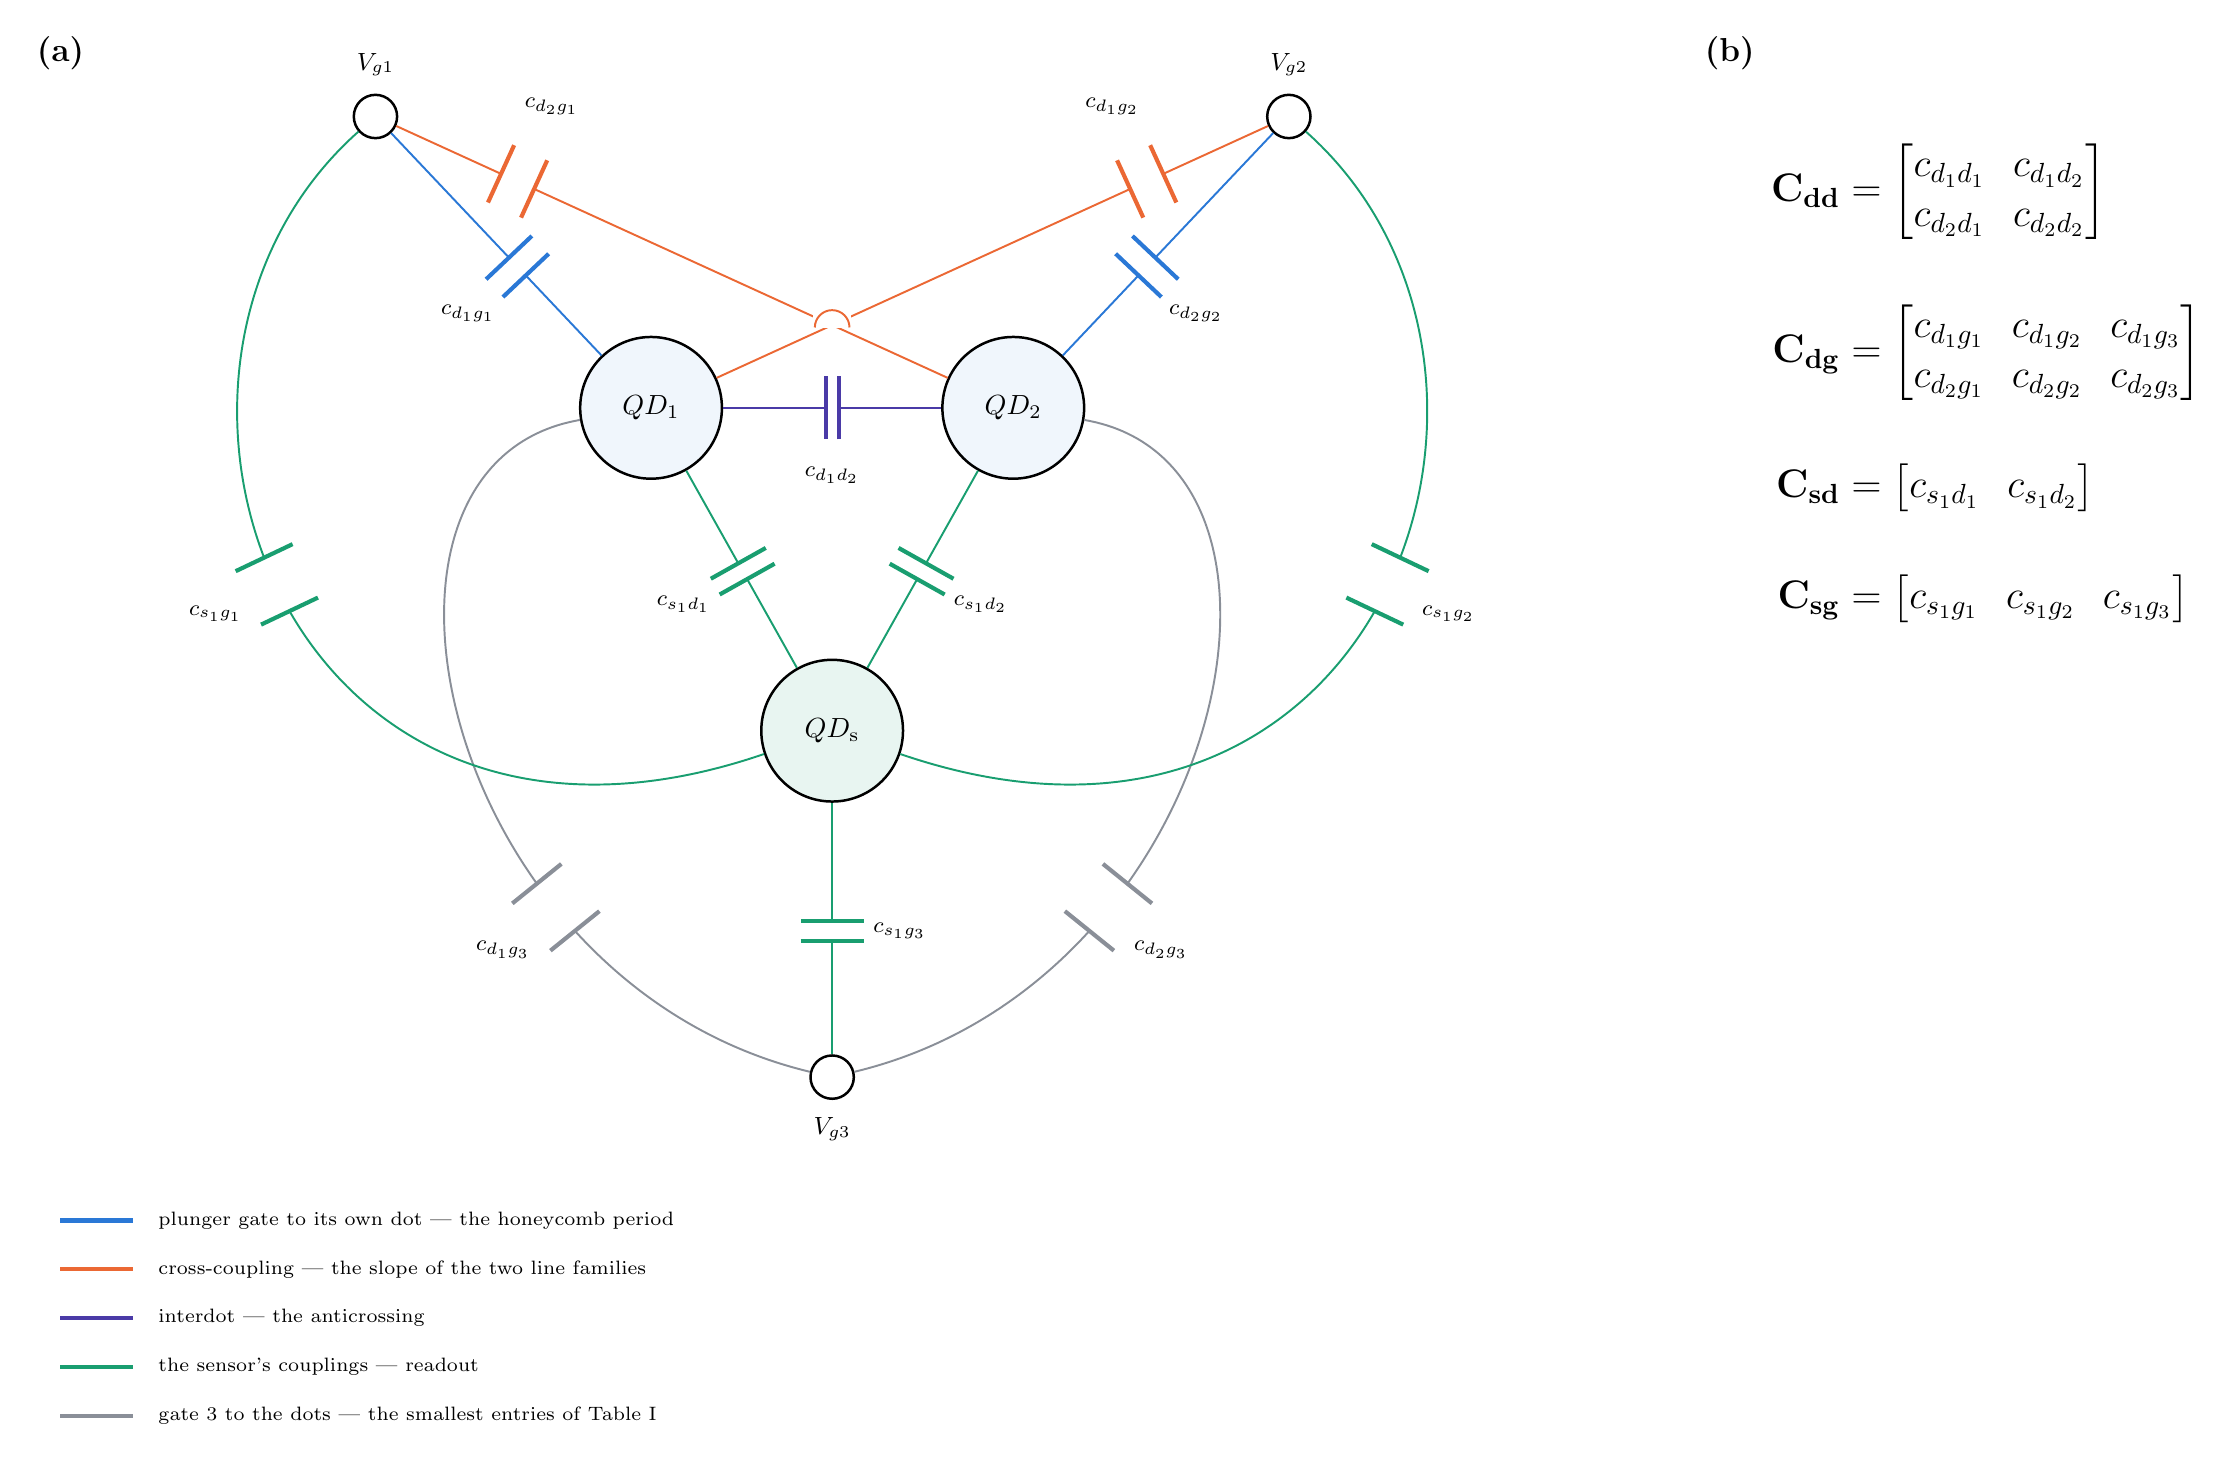
\begin{tikzpicture}[
    island/.style = {circle, draw, line width=0.9pt, minimum size=18mm,
                     fill=cPrim!7, inner sep=0pt},
    sensor/.style = {circle, draw, line width=0.9pt, minimum size=18mm,
                     fill=cSens!10, inner sep=0pt},
    gate/.style   = {circle, draw, line width=0.9pt, minimum size=5.5mm,
                     fill=white, inner sep=0pt},
    wire/.style   = {line width=0.7pt},
    lab/.style    = {font=\footnotesize, inner sep=1.4pt,
                     fill=white, fill opacity=0.92,
                     text opacity=1},
  ]

  % ── nodes ──────────────────────────────────────────────────────────────
  \node[gate]   (g1) at (-5.8,  4.8) {};
  \node[gate]   (g2) at ( 5.8,  4.8) {};
  \node[gate]   (g3) at ( 0.0, -7.4) {};
  \node[island] (d1) at (-2.3,  1.1) {$QD_1$};
  \node[island] (d2) at ( 2.3,  1.1) {$QD_2$};
  \node[sensor] (s1) at ( 0.0, -3.0) {$QD_\mathrm{s}$};

  \node[font=\small] at ($(g1)+(0,0.66)$) {$V_{g1}$};
  \node[font=\small] at ($(g2)+(0,0.66)$) {$V_{g2}$};
  \node[font=\small] at ($(g3)+(0,-0.66)$) {$V_{g3}$};

  % ── the capacitor symbol ───────────────────────────────────────────────
  % #1,#2  two points a short way apart ON the wire: the plates are drawn
  %        square to the line joining them, so this works on a curve as well
  %        as on a straight, and the white stroke opens the gap between them.
  % #3     the label, #4 where it sits
  \def\platecolour{black}
  \newcommand{\plates}[5]{%
    \draw[white, line width=2.2pt] (#1) -- (#2);
    \draw[line width=1.5pt, \platecolour] ($(#1)!0.40cm!90:(#2)$) --
                            ($(#1)!0.40cm!-90:(#2)$);
    \draw[line width=1.5pt, \platecolour] ($(#2)!0.40cm!90:(#1)$) --
                            ($(#2)!0.40cm!-90:(#1)$);
    \coordinate (mid) at ($(#1)!0.5!(#2)$);
    \node[lab] at ($(mid)!#5!#4:(#2)$) {$c_{#3}$};
  }

  % ── every wire first, so no plate is drawn over by a later line ────────
  \draw[wire, cPrim] (g1) -- (d1);
  \draw[wire, cPrim] (g2) -- (d2);
  \draw[wire, cCross, name path=cross1] (g1) -- (d2);
  \draw[wire, cCross, name path=cross2] (g2) -- (d1);
  \draw[wire, cInter] (d1) -- (d2);
  \draw[wire, cSens] (d1) -- (s1);
  \draw[wire, cSens] (d2) -- (s1);
  \draw[wire, cSens] (g3) -- (s1);
  \draw[wire, cWeak] (d1) .. controls (-6.4,0.4) and (-5.0,-6.2) .. (g3);
  \draw[wire, cWeak] (d2) .. controls ( 6.4,0.4) and ( 5.0,-6.2) .. (g3);
  \draw[wire, cSens] (g1) .. controls (-9.4,1.6) and (-7.0,-5.4) .. (s1);
  \draw[wire, cSens] (g2) .. controls ( 9.4,1.6) and ( 7.0,-5.4) .. (s1);

  % ── the hop, at the one crossing the graph cannot avoid ────────────────
  % g1--d2 and g2--d1 meet on the axis of symmetry; the point is taken from
  % the path rather than guessed.
  \path[name intersections={of=cross1 and cross2, by=xing}];
  \fill[white] ($(xing)+(-0.24,-0.04)$) rectangle ($(xing)+(0.24,0.30)$);
  \draw[wire, cCross] ($(xing)+(-0.22,-0.03)$) arc (180:0:0.22);

  % ── the plates ─────────────────────────────────────────────────────────
  \path (g1) -- (d1) coordinate[pos=0.56] (a1) coordinate[pos=0.64] (a2);
  {\def\platecolour{cPrim}\plates{a1}{a2}{d_1g_1}{-90}{0.86cm}}
  \path (g2) -- (d2) coordinate[pos=0.56] (b1) coordinate[pos=0.64] (b2);
  {\def\platecolour{cPrim}\plates{b1}{b2}{d_2g_2}{90}{0.86cm}}

  \path (g1) -- (d2) coordinate[pos=0.19] (c1) coordinate[pos=0.25] (c2);
  {\def\platecolour{cCross}\plates{c1}{c2}{d_2g_1}{90}{1.05cm}}
  \path (g2) -- (d1) coordinate[pos=0.19] (e1) coordinate[pos=0.25] (e2);
  {\def\platecolour{cCross}\plates{e1}{e2}{d_1g_2}{-90}{1.05cm}}

  \path (d1) -- (d2) coordinate[pos=0.47] (f1) coordinate[pos=0.53] (f2);
  {\def\platecolour{cInter}\plates{f1}{f2}{d_1d_2}{-90}{0.86cm}}
  \path (d1) -- (s1) coordinate[pos=0.47] (h1) coordinate[pos=0.55] (h2);
  {\def\platecolour{cSens}\plates{h1}{h2}{s_1d_1}{-90}{0.86cm}}
  \path (d2) -- (s1) coordinate[pos=0.47] (i1) coordinate[pos=0.55] (i2);
  {\def\platecolour{cSens}\plates{i1}{i2}{s_1d_2}{90}{0.86cm}}
  \path (g3) -- (s1) coordinate[pos=0.45] (j1) coordinate[pos=0.53] (j2);
  {\def\platecolour{cSens}\plates{j1}{j2}{s_1g_3}{-90}{0.86cm}}

  \path (d1) .. controls (-6.4,0.4) and (-5.0,-6.2) .. (g3)
        coordinate[pos=0.68] (k1) coordinate[pos=0.74] (k2);
  {\def\platecolour{cWeak}\plates{k1}{k2}{d_1g_3}{-90}{0.86cm}}
  \path (d2) .. controls (6.4,0.4) and (5.0,-6.2) .. (g3)
        coordinate[pos=0.68] (l1) coordinate[pos=0.74] (l2);
  {\def\platecolour{cWeak}\plates{l1}{l2}{d_2g_3}{90}{0.86cm}}
  \path (g1) .. controls (-9.4,1.6) and (-7.0,-5.4) .. (s1)
        coordinate[pos=0.46] (m1) coordinate[pos=0.52] (m2);
  {\def\platecolour{cSens}\plates{m1}{m2}{s_1g_1}{-90}{0.86cm}}
  \path (g2) .. controls (9.4,1.6) and (7.0,-5.4) .. (s1)
        coordinate[pos=0.46] (n1) coordinate[pos=0.52] (n2);
  {\def\platecolour{cSens}\plates{n1}{n2}{s_1g_2}{90}{0.86cm}}

  \node[font=\bfseries\large] at (-9.8, 5.6) {(a)};

  % ── (b) the matrices, in full ──────────────────────────────────────────
  \node[anchor=north west, font=\Large] at (11.8, 4.6) {$\begin{aligned}
      \mathbf{C}_{\mathbf{dd}} &=
        \begin{bmatrix}
          c_{d_1 d_1} & c_{d_1 d_2} \\
          c_{d_2 d_1} & c_{d_2 d_2}
        \end{bmatrix} \\[18pt]
      \mathbf{C}_{\mathbf{dg}} &=
        \begin{bmatrix}
          c_{d_1 g_1} & c_{d_1 g_2} & c_{d_1 g_3} \\
          c_{d_2 g_1} & c_{d_2 g_2} & c_{d_2 g_3}
        \end{bmatrix} \\[18pt]
      \mathbf{C}_{\mathbf{sd}} &=
        \begin{bmatrix}
          c_{s_1 d_1} & c_{s_1 d_2}
        \end{bmatrix} \\[18pt]
      \mathbf{C}_{\mathbf{sg}} &=
        \begin{bmatrix}
          c_{s_1 g_1} & c_{s_1 g_2} & c_{s_1 g_3}
        \end{bmatrix}
    \end{aligned}$};
  \node[font=\bfseries\large] at (11.4, 5.6) {(b)};


  % ── the key ────────────────────────────────────────────────────────────
  % Identity is never colour alone: every wire carries its own label as well.
  \begin{scope}[shift={(-9.8,-8.6)}]
    \foreach \col/\txt [count=\i] in {%%
        cPrim/{plunger gate to its own dot \textemdash\ the honeycomb period},
        cCross/{cross-coupling \textemdash\ the slope of the two line families},
        cInter/{interdot \textemdash\ the anticrossing},
        cSens/{the sensor's couplings \textemdash\ readout},
        cWeak/{gate 3 to the dots \textemdash\ the smallest entries of Table I}}
      {
        \draw[\col, line width=1.6pt]
          (0, -0.62*\i) -- ++(0.92,0);
        \node[anchor=west, font=\scriptsize, text=black]
          at (1.12, -0.62*\i) {\txt};
      }
  \end{scope}

\end{tikzpicture}
\end{document}
